\begin{savequote}[8cm]
\textlatin{Neque porro quisquam est qui dolorem ipsum quia dolor sit amet, consectetur, adipisci velit...}

There is no one who loves pain itself, who seeks after it and wants to have it, simply because it is pain...
  \qauthor{--- Cicero's \textit{de Finibus Bonorum et Malorum}}
\end{savequote}

\chapter{\label{ch:7-com}Centre-of-momentum variables} 

\section{Introduction}
Significant efforts have been devoted to measuring Charge-Parity (CP) violation in the neutrino sector through long-baseline (LBL) experiments. 
\blue{In these experiments, CP violation is quantified by the difference between neutrino oscillation and anti-neutrino oscillation. 
LBL experiments quantify $\dcp$ by comparing the energy spectra of $\nue$ and $\nuebar$ oscillated from $\numu$ and $\numubar$, respectively.
There are two major challenges to this measurement. 
Firstly, the far detector of an LBL experiment is by design hundreds of kilometres away from the neutrino source, which unavoidably lead to low statistics.
Secondly, as the energy of each incoming neutrino is unknown and thus the type of the individual neutrino bound-nucleon interaction is also unknown, oscillation predictions have to take the form of energy spectra for a chosen final state topologies.
Accurate $\dcp$ measurements heavily depend on neutrino interaction models estimating contributions of different neutrino-nucleon interactions to final-state topologies~\cite{NuSTEC:2017hzk}.
Large-scale experiments, such as Hyper-Kamiokande~\cite{Hyper-Kamiokande:2018ofw} and the Deep Underground Neutrino Experiment (DUNE)~\cite{DUNE:2015lol,DUNE:2016evb,DUNE:2016hlj,DUNE:2016rla,DUNE:2021tad}, address this challenge by constructing gigantic far detectors to increase event rates.
To match the reduction of statistical uncertainties, it is critical to develop advanced neutrino interaction models or to better constrain existing ones to minimize the systematic uncertainties.}

To better understand the complex neutrino-nucleus interactions, new or upgraded experiments with sophisticated detectors have commenced to explore a larger interaction kinematic phase space and to collect a significantly larger amount of data. 
For instance, the Tokai-to-Kamioka (T2K) experiment~\cite{T2K:2011qtm} has upgraded its near detector (ND) and started data collection in June 2024. 
The Super Fine-Grain Detector (SFGD), part of the T2K ND upgrade~\cite{T2K:2019bbb}, provides improved proton detection with lower thresholds, higher resolution, and greater efficiency. 
Meanwhile, the Short-baseline Near Detector (SBND)~\cite{MicroBooNE:2015bmn} has also begun operations in 2024. 
It is a new LArTPC with an active mass of 112 ton placed at $110$ m from the neutrino source. 
Due to its large active mass and proximity to the source,  it is expected to collect a huge number of neutrino interaction events each year.  
On one hand, the expanded kinematic phase space allows for measuring new variables. 
On the other, the influx of high-quality data offers an ideal testing ground for novel measurement techniques.
Taking advantage of these advancements, it is timely to explore new ideas involving pions in the final states, given the broad energy spectrum of the DUNE beamline, which includes substantial contributions from resonance production comparable to quasi-elastic interactions, 

One effective method of utilizing the near detector data is to constrain model parameters through tuning.
Successful examples~\cite{GENIE:2021zuu,GENIE:2021wox,GENIE:2022qrc} have shown improved data-Monte Carlo (MC) agreement after tuning existing models using various combinations of measurements from different experiments. 
However, the neutrino-nucleus interaction is a convolution of multiple processes: the nucleon initial state (IS), the neutrino-nucleon interaction, and final state interactions (FSI). 
Many variables are affected by all these processes, making it challenging to study the different models in isolation. 
Nuclear effects, such as IS and FSI, occur within the nucleus and remain unobservable with current detectors, making them a major source of systematic uncertainties.
Cleverly constructed variables, such as Transverse Kinematic Imbalance (TKI)~\cite{Lu:2015hea, Lu:2015tcr} or Generalized Kinematic Imbalance (GKI)~\cite{MicroBooNE:2023krv}, are sensitive to nuclear effects, and past measurements have successfully constrained models~\cite{GENIE:2024ufm}. 
While TKI is sensitive to both IS and FSI, except $\dat$, which is predominantly sensitive to FSI but is affected by small uncertainties in the neutrino direction, new variables like $\plong$ \cite{Baudis:2023tma} are designed to be sensitive to specific nuclear effects, such as the removal energy. 

Having more specialized measurements, like $\plong$, can further fine-tune our models, especially in light of the improved detection capabilities. 
This work proposes a new set of variables, called center-of-momentum (COM) variables, for charge current single pion single proton ($\ccopiop$) events, timely for the increasingly precise measurements with pions in the final states
COM variables enable more focused studies of FSI by differentiating between FSI models independently of IS models.

This paper will elaborate on the concept of the COM variables and present MC analysis results focusing on the COM angle and demonstrating its ability to distinguish FSI models and its independence from IS.

\section{The COM Variables}
\label{sec:com}
When a neutrino has sufficient energy, it can excite a nucleon into a resonance state, for example the $\deltapp$. 
This process is referred to as a resonance (RES) interaction.
Since $\deltapp$ is one of the most commonly observed resonances in neutrino experiments, this work focuses on it as an example.
Nevertheless, the concept presented here is equally applicable to other resonances, and the methodology can be easily generalized.

The resonance decays rapidly, before leaving the nucleus, via the process
\begin{equation}
	\deltapp \rightarrow \pip + \p.
\end{equation}
In the $\deltapp$ rest frame, as illustrated on the top left in Fig.~\ref{fig:COM-diagram}, the kinematics of this two-body decay are well-defined and the proton and pion are emitted back-to-back.
The pion decay angle, $\thetapidel$, is defined as the angle between $\vecppirest$ and the $x$-axis, which is taken to align with $\vecpdel$, the momentum of $\deltapp$ in the lab frame. 
$\thetapidel$ is a resonance property that follows an underlying distribution defined by various models~\cite{Rein:1987cb,Kabirnezhad:2017jmf,Kabirnezhad:2020wtp,Kabirnezhad:2022znc}.

\begin{figure}[ht!]
    \centering
    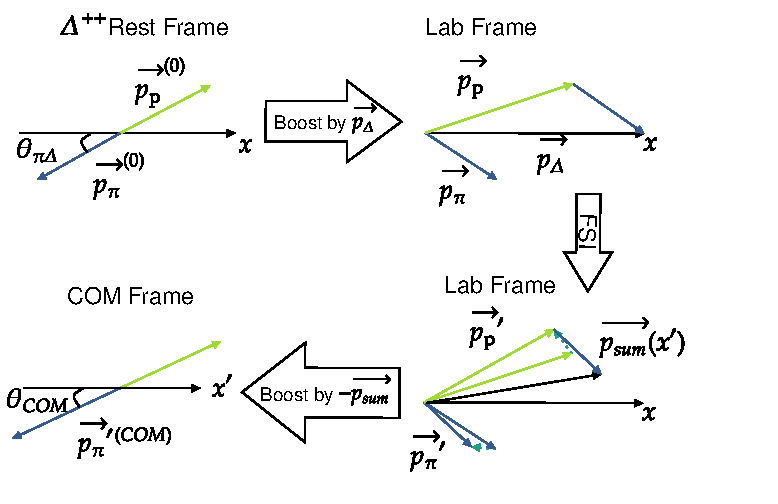
\includegraphics[width=\linewidth]{COM-diagram.pdf}
    \caption{Schematic illustration of the COM angle. \blue{Without FSI, $\vecpsum=\vecpdel$ and the lab frame and the $\deltapp$ rest frame can be transformed into each other by $\vecpdel$. With FSI, $\vecpsum \neq \vecpdel$, the $\deltapp$ rest frame is not accessible, but the lab frame can be boosted into the COM frame using $\vecpsum$. Hence, the major difference of the COM frame from the $\deltapp$ rest frame is caused by FSI.} }
    \label{fig:COM-diagram}
\end{figure}

The kinematics in the lab frame are related to those in the $\deltapp$ rest frame by a boost with $\vecpdel$, as depicted on the top right of Fig.~\ref{fig:COM-diagram}. 
Without FSI, $\vecpdel$ equals the sum of $\vecpp$ and $\vecppi$.
However, the target materials of modern day detectors are mainly comprised of nucleus with multiple nucleons and FSI alters the kinematics of the hadrons considerably, as illustrated by the dotted arrows in the bottom right of Fig.~\ref{fig:COM-diagram}.

The altered momenta, $\vecppp$ and $\vecppip$, are the ones measured by detectors. 
Their sum generally differs from $\vecpdel$.
Thus, the $\deltapp$ rest frame with its simple kinematic relations becomes inaccessible.
Nevertheless, the system can be boosted to the proton-pion COM frame using $\vecpsum$, as depicted in the bottom left of Fig.~\ref{fig:COM-diagram}, where the $x^{\prime}$-axis is taken to align with the $\vecpsum$ direction in the lab frame.
Similarly, a pion decay angle, $\thetacom$, can be defined between, $\vecppicom$, the pion momentum in the COM frame, and the $x^{\prime}$-axis.
Due to FSI, $\thetacom$ typically differs from $\thetapidel$. 

The COM frame coincides with the $\deltapp$ rest frame only in the absence of FSI.
Thus, the strength of FSI dictates the deviation of $\thetacom$ from $\thetapidel$. 
In practice, the measured $\thetacom$ serves as a probe for studying FSI. 
$\thetapidel$, being a rest-frame property of $\deltapp$, is independent of the resonance's momentum, neutrino energy, and IS.
In neutrino event generators, $\thetacom$ deviates from $\thetapidel$ only due to FSI, which is independent of neutrino energy and IS.
Therefore, $\thetacom$ retains these important independencies.
\blue{As different resonances could have different decay properties, $\thetaR$, the similarly defined pion decay angle of a higher resonance, $R$, generally differs from $\thetapidel$. 
Hence, $\thetacom$, a superposition of $\thetapidel$ and all possible $\thetaR$, will deviate from $\thetapidel$, when more resonances become energetically possible with an increase in neutrino energy. 
This deviation will be further elaborated in the Sec.~\ref{sec:dis}.}

Moreover, the total energy in the COM frame will be equal to the mass of the resonance in the absence of FSI.
Cutting on events with total energy far from the rest mass peak of the resonance will select events with minimal FSI effects, such as the $\nu$-H events. 
However, this work will focus on the COM angle only, and analysis on the total energy will be conducted in future works.

Up to this point, the discussion of resonance decay has been entirely general and can thus be applied to and validated by various experiments, including hadron scattering measurements. 
However, there are features specific to neutrino experiments. 
First, the resonance is generated through neutrino-nucleon interactions, which involve both vector and axial currents. 
Second, the interaction occurs within the nuclear medium. 
This work focuses on the latter, with the application of COM variables to the former reserved for future research.

While the COM angle may appear conceptually similar to the reconstructed Adler angle, $\thetaadt$, in neutrino experiments~\cite{Sanchez:2015yvw}, there are significant differences. 
Notably, the COM frame is reconstructed exclusively from hadronic kinematics, whereas the reconstructed Adler frame relies on leptonic kinematics and assumes stationary nucleons. 
Consequently, the reconstruction of the Adler frame is implicitly influenced by IS effects, whereas the COM frame's hadronic variables are impacted by final state interactions (FSI). 
Therefore, $\thetaadt$, being a hadronic variable in the Adler frame, is influenced by both IS and FSI. 
Additionally, the necessity of reconstructing the neutrino energy renders $\thetaadt$ sensitive to neutrino flux uncertainties, which are among the largest systematic uncertainties in neutrino measurements~\cite{T2K:2019yqu,T2K:2021naz,MicroBooNECollaboration:2024gvg,NOvA:2023uxq,MINERvA:2022djk}.


\section{Analysis result}
\label{sec:ana}

In the absence of existing measurements of the COM angle, MC studies were conducted to evaluate its potential advantages.
MC samples were generated using \genie \cite{Andreopoulos:2009rq, GENIE:2021npt} for T2K beam and target. 
Several \genie tunes were compared, with the model details for each tune summarized in Table~\ref{tab:genie-tunes}. 
Each sample consists of $600,000$ muon neutrino events, and a selection of charge current single pion and single proton ($\numuccopiop$) events was used to generate the plots.

\begin{table}[h]
    \centering
    \begin{tabular}{c|c|c|c|c|c}
     CMC                  &  IS  &  QE                & 2p2h         & RES & FSI\\
     \colrule
     G18\_01a\_02\_11b    &  RFG         &   LS               & Dytman       & RS  & hA\\
     G18\_02a\_02\_11b    &  RFG         &   LS               & Dytman       & BS  & hA\\
     G18\_10a\_02\_11b\footnote{The \genie default uses local Fermi gas instead.}    
                          &  CFG         &  Valencia          & Nieves       & BS  & hA\\
     G18\_10b\_02\_11b    &  LFG         &  Valencia          & Nieves       & BS  & hN\\
     G24\_20i\_00\_000    &  SF-CFG      &  Valencia          & SuSAv2       & BS  & hA\\
     G24\_20i\_06\_22c    &  SF-CFG      &  Valencia          & SuSAv2       & BS  & hA(tuned)\\
    \end{tabular}
    \caption{The four nuclear IS models are relativistic Fermi gas (RFG), local Fermi gas (LFG), correlated Fermi gas (CFG), spectral-function-like CFG (SF-CFG)~\cite{sfcfg-talk,sfcfg-GitHubCommit,GENIE:2021npt}. 
    The respective cross-section models are: 1) Quasielastic (QE) - Llewellyn-Smith (LS)~\cite{LlewellynSmith:1971uhs} and Valencia~\cite{Nieves:2004wx}; 2) 2p2h - Dytman~\cite{genie:2p2h-dytman}, Nieves~\cite{Nieves:2011pp} and SuSAv2~\cite{Gonzalez-Jimenez:2014eqa}; 3) RES - Rein-Sehgal~\cite{Rein:1980wg} and Berger-Sehgal~\cite{Berger:2007rq}. 
    The FSI models are the built-in \genie models~\cite{Andreopoulos:2015wxa}, INTRANUKE hA and hN. Note that in \texttt{G24\_20i\_06\_22c}~\cite{GENIE:2024ufm}, the hA model has been tuned using TKI data, resulting in parameters that differ from the default hA.}
    \label{tab:genie-tunes}
\end{table}


\begin{figure}[ht!]
    \centering
    \begin{subfigure}[ht!]{\scfigwid\textwidth}
        \centering
        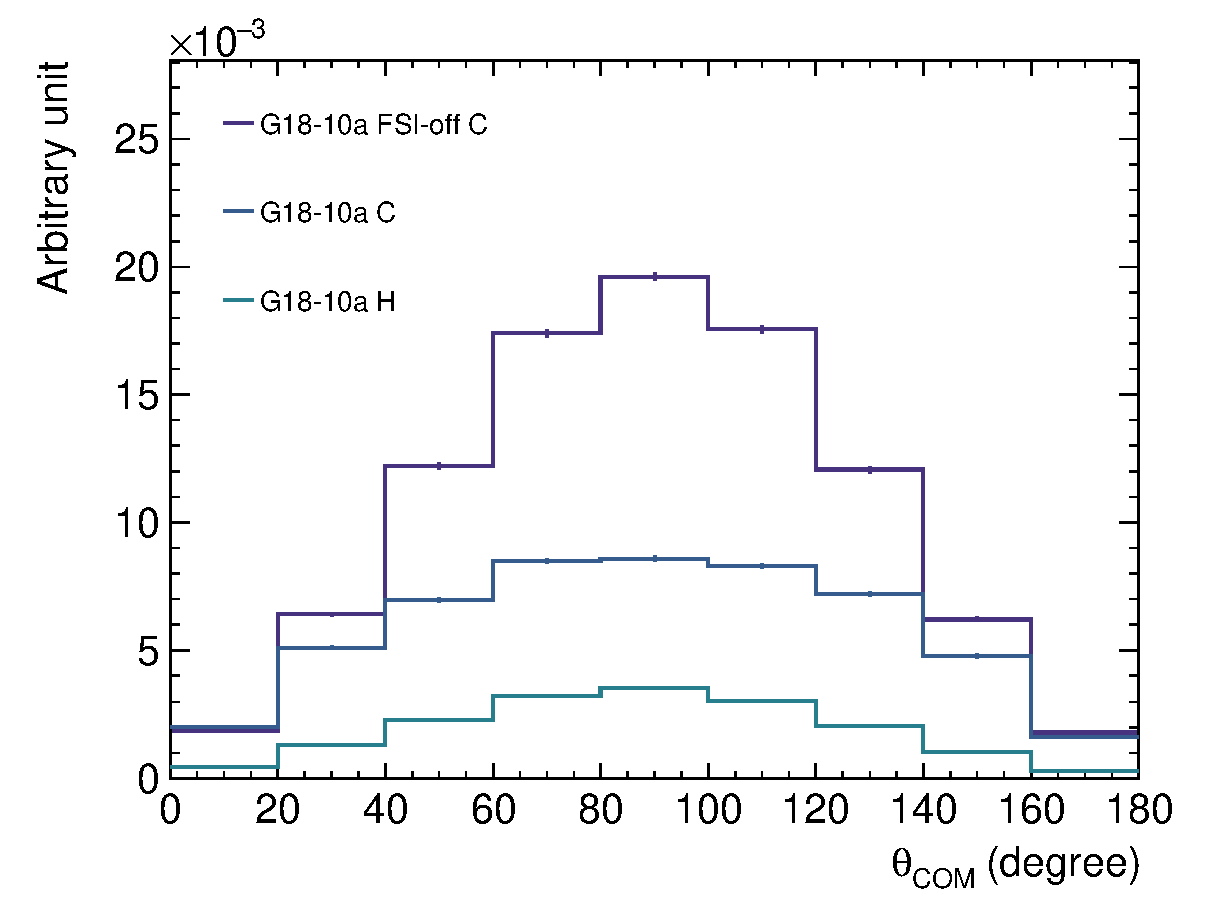
\includegraphics[width=\textwidth]{xnorm-CH_da_tan.eps} \\
        \caption{Cross-section normalized comparisons with FSI on/off for carbon and hydrogen with \texttt{G18\_10a\_02\_11b}.}
        \label{subfig:fsi-comp-chof}
    \end{subfigure}
    \begin{subfigure}[ht!]{\scfigwid\textwidth}
        \centering
        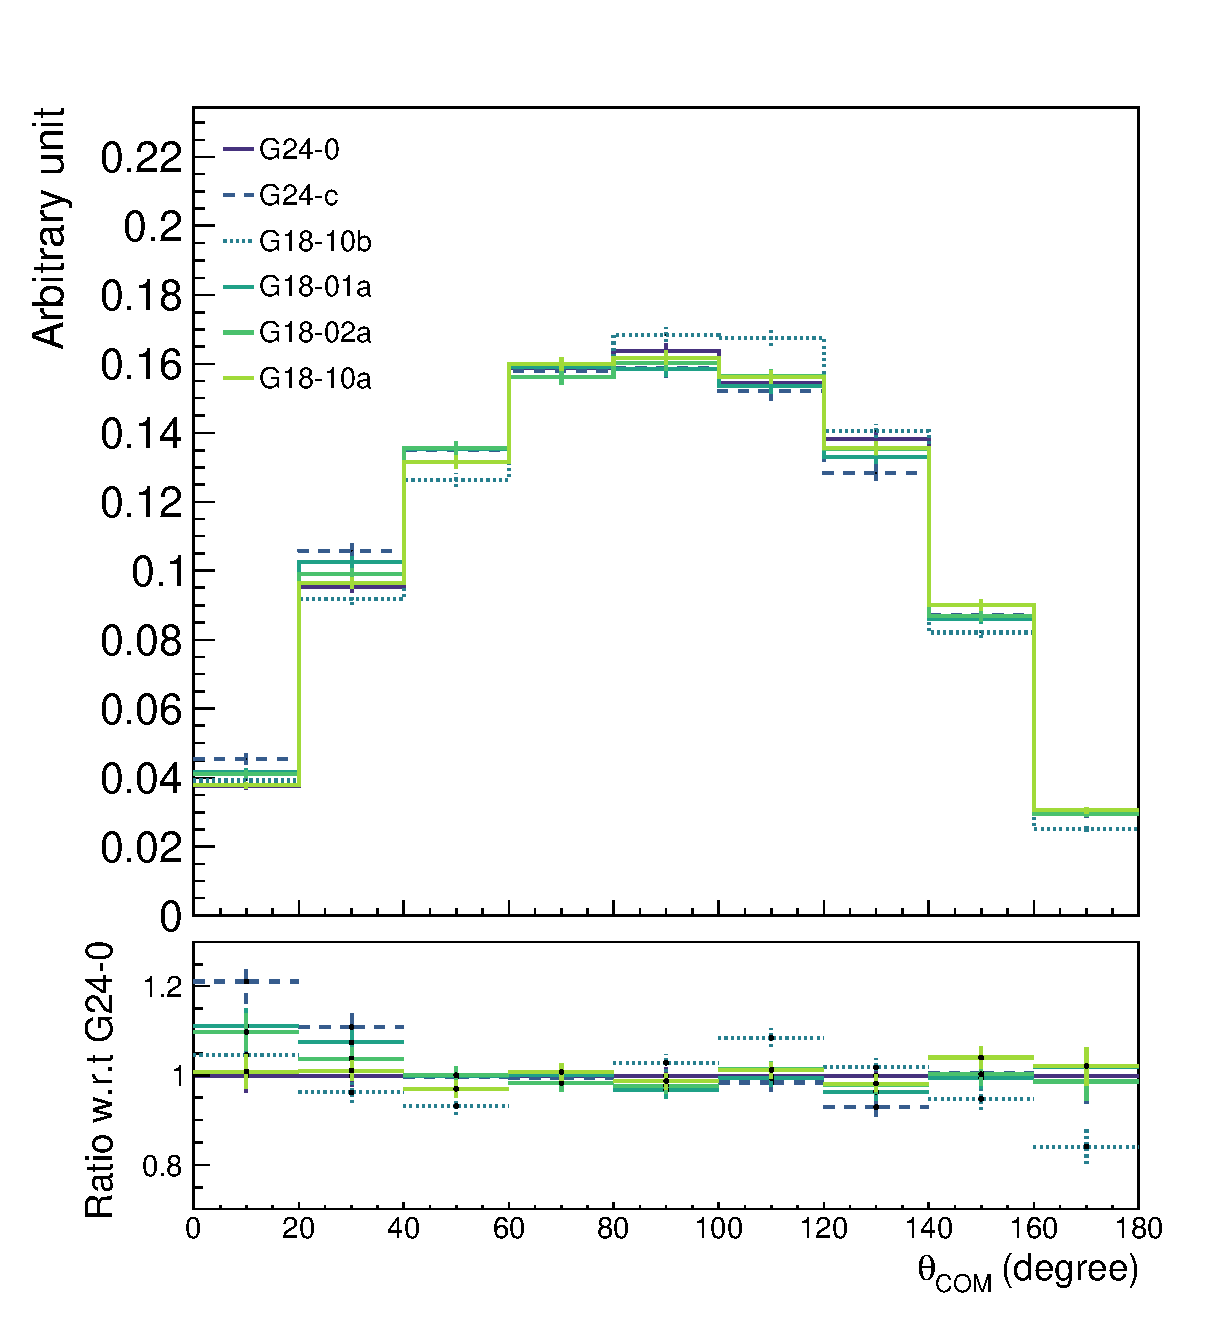
\includegraphics[width=\textwidth]{anorm-mod-ratio-_da_tan.eps}
        \caption{Area normalized comparisons for different tunes with FSI on for carbon. }
        \label{subfig:fsi-comp-gt}
    \end{subfigure}
    \caption{\blue{$\thetacom$ distribution comparisons using T2K flux on different nuclei and with multiple \genie configuations.} }
    \label{fig:fsi-comp}
\end{figure}

As illustrated in Fig.~\ref{fig:fsi-comp} (a), enabling or disabling FSI has a significant effect on the $\thetacom$ cross-section as expected.
More critically, Fig.~\ref{fig:fsi-comp} (b) shows that changing the underlying FSI model from hA (10a) to hN (10b) or from hA (10a) to hA (tuned, G24-c) results in a noticeable variation in the $\thetacom$ cross-section. 
In contrast, although numerous combinations of IS, QE, 2p2h, and RES models were tested, configurations using the hA FSI model produced nearly identical cross-sections.
This demonstrates the potential of $\thetacom$ to distinguish between different FSI models, independent of many other factors.


To further examine the independence from IS of $\thetacom$, the cross-section shape of $\nu$-C (with FSI on and off) is compared to that of $\nu$-H. 
The $\nu$-H interaction is free from any nuclear effects, while $\nu$-C without FSI reflects the impact of IS, including carbon removal energy and Fermi motion. 
When FSI is on, the full nuclear effects—both IS and FSI—are present. 
Fig.~\ref{subfig:ch-comp-com-cc1pi1p} shows that FSI has a substantial impact on the cross-section shape, as expected. 
The near overlap of the $\nu$-H and $\nu$-C (FSI-off) curves provides strong evidence for the proposed independence of $\thetacom$ from IS effects.

\begin{figure}
    \centering
    \begin{subfigure}[ht!]{\scfigwid\textwidth}
        \centering
        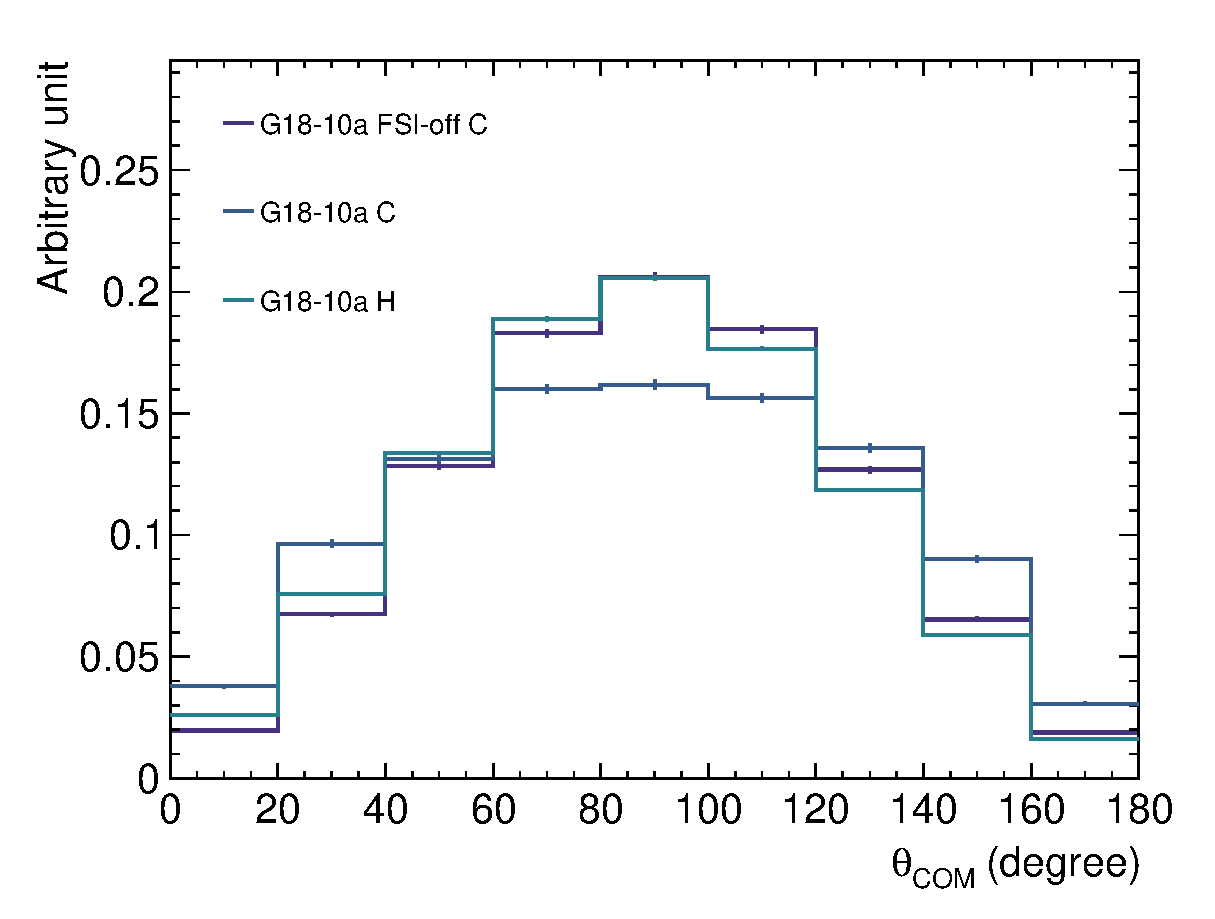
\includegraphics[width=\textwidth]{anorm-CH_da_tan.eps}     
        \caption{$\thetacom$ - general $\numuccopiop$.}
        \label{subfig:ch-comp-com-cc1pi1p}
    \end{subfigure}
          % \hfill
    \begin{subfigure}[ht!]{\scfigwid\textwidth}
        \centering
        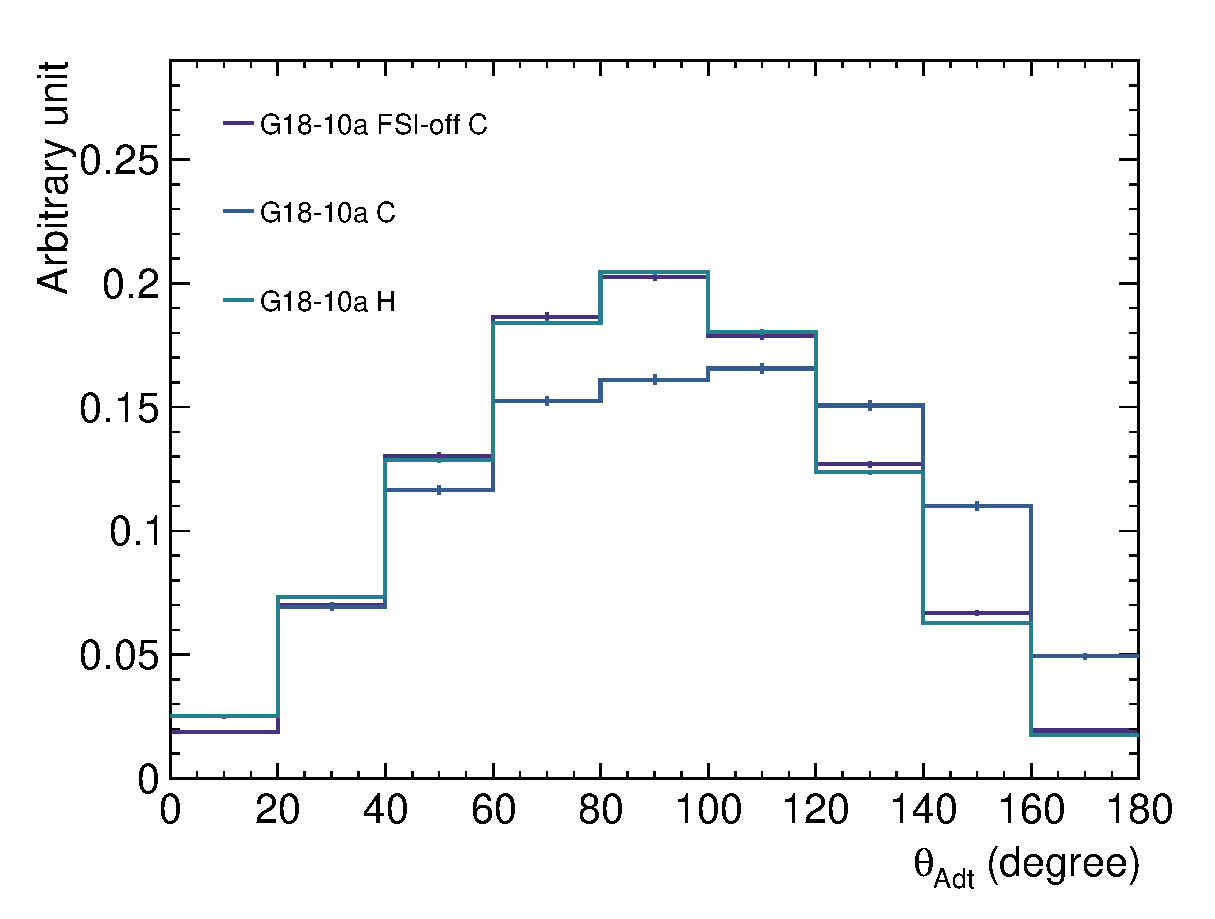
\includegraphics[width=\textwidth]{anorm-CH_adt.eps}        
        \caption{$\thetaadt$ - general $\numuccopiop$.}
        \label{subfig:ch-comp-adt-cc1pi1p}
    \end{subfigure} 
    \caption{\blue{Area normalized comparisons for FSI on/off for carbon and hydrogen with \texttt{G18\_10a\_02\_11b} between $\thetacom$ and $\thetaadt$ using T2K flux and target.}  with the bottom row has a more stringent selection to restrict the resonance to be $\deltapp$.}
    \label{fig:ch-comp}
\end{figure}

Although $\thetacom$ is conceptually similar to the reconstructed Adler angle, $\thetaadt$, the latter is additionally influenced by IS effects. 
However, Fig.~\ref{subfig:ch-comp-adt-cc1pi1p}  suggests that the $\nu$-H and $\nu$-C (FSI-off) curves remain nearly as close as in Fig.~\ref{subfig:ch-comp-com-cc1pi1p}. 
When a stricter selection is made to select only events involving $\deltapp$ as shown in Fig.~\ref{fig:ch-comp-dpp} in Appendix, the small difference in $\thetacom$ reduces further while the two curves deviate slightly more in $\thetaadt$. 
This suggests that in the absence of FSI, $\thetacom$ could be a better construction of $\theta$ than $\thetaadt$. 

Nevertheless, the small difference between the two curves for $\thetaadt$ indicates that despite IS dependence, IS does not significantly distort the shape of $\thetaadt$ appreciably.
This observation could challenge the claimed IS independence of $\thetacom$, as it might be due to the relatively minor influence of IS. 
To further examine this, a stress test was conducted by varying the removal energy of carbon across a wide range, even to unphysical levels, to assess its effect on the shapes of $\thetacom$ and $\thetaadt$. 
The results are presented in Fig.~\ref{fig:ermc-comp}.

\begin{figure}[ht!]
    \centering
    \begin{subfigure}[ht!]{\scfigwid\textwidth}
        \centering
        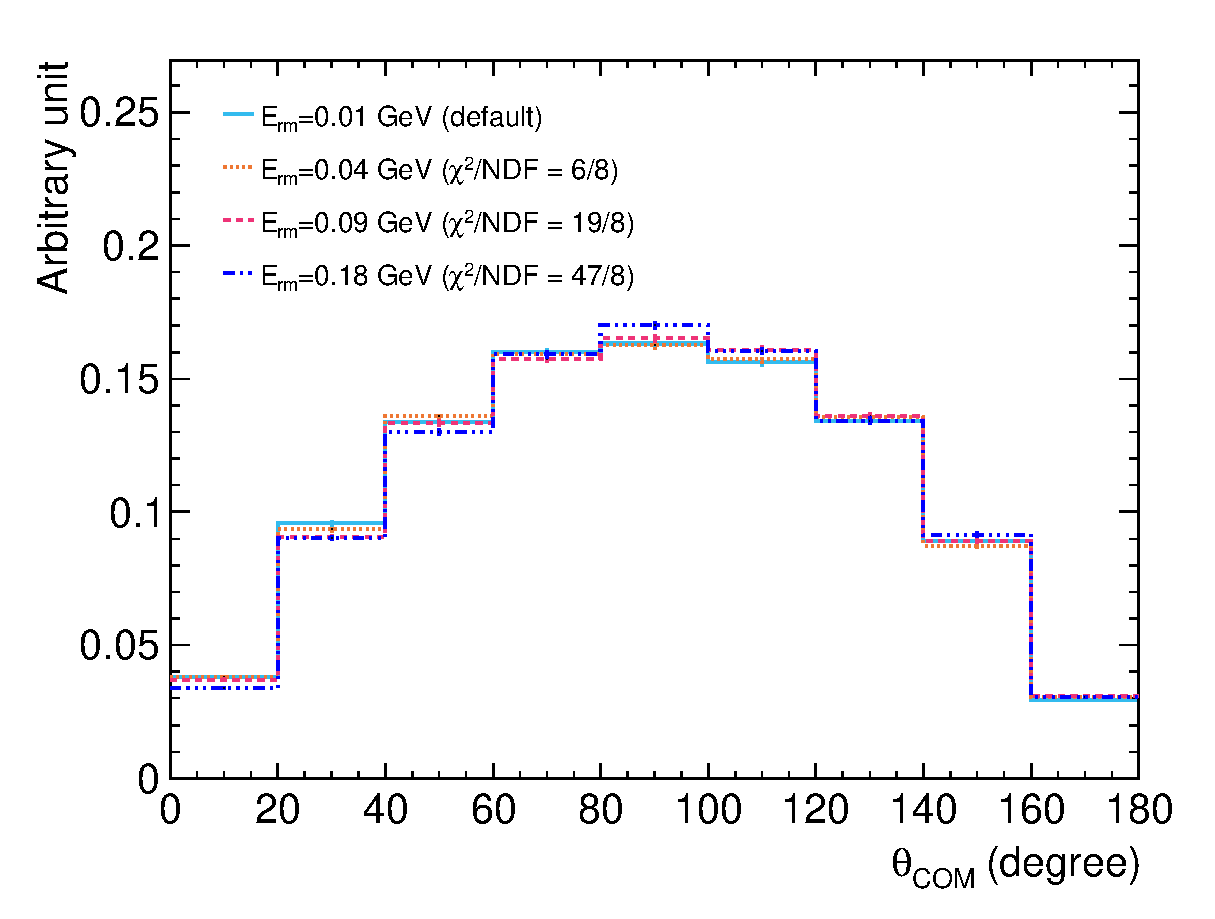
\includegraphics[width=\textwidth]{anorm-nuc_da_tan.eps}\\
        \caption{$\thetacom$}
        \label{subfig:ermc-comp-com}
    \end{subfigure}
    \begin{subfigure}[ht!]{\scfigwid\textwidth}
        \centering
        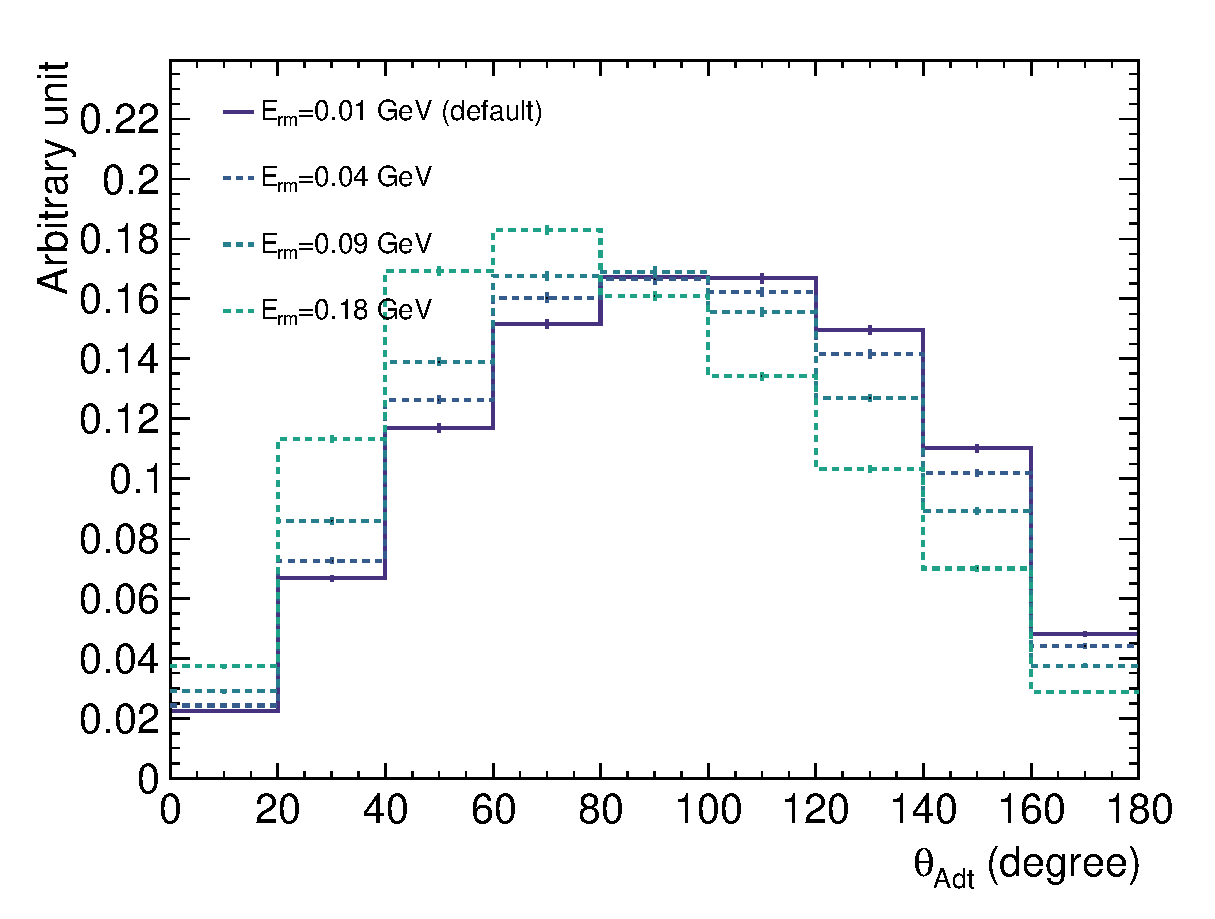
\includegraphics[width=\textwidth]{anorm-nuc_adt.eps}
        \caption{$\thetaadt$}
        \label{subfig:ermc-comp-adt}
    \end{subfigure}
        
    \caption{Area normalized comparisons for different removal energies, $E_{\textrm{rm}}$, with T2K flux.}
    \label{fig:ermc-comp}
\end{figure}

As seen in Fig.~\ref{fig:ermc-comp}, variations in the removal energy ($E_{\textrm{rm}}$) do not affect $\thetacom$ at all. 
In contrast, the $\thetaadt$ peak exhibits a noticeable shift, along with a gradual change in its shape.
These results confirm that $\thetacom$ is independent of IS effects, while $\thetaadt$ exhibits IS dependence, as predicted.

Another important feature of $\thetacom$ is its independence from neutrino energy. 
Fig.~\ref{fig:enu-comp} illustrates this behavior. 
The $\thetacom$ distribution shapes remain largely consistent for $\enu$ values between $0.5~\gev$ and $2.0~\gev$ across most angles.
However, deviations become more pronounced at smaller angles. 
As $\enu$ increases to $5\gev$, a noticeable rise is observed in the small-angle region, likely due to the onset of a higher doubly positive resonance. 
If the analysis is limited to $\deltapp$ as in Fig.~\ref{fig:enu-comp}(b), it is encouraging to observe that the different curves converge, confirming the independence of $\thetacom$ from $\enu$.

\begin{figure}[ht!]
    \centering
    \begin{subfigure}[ht!]{\scfigwid\textwidth}
        \centering
        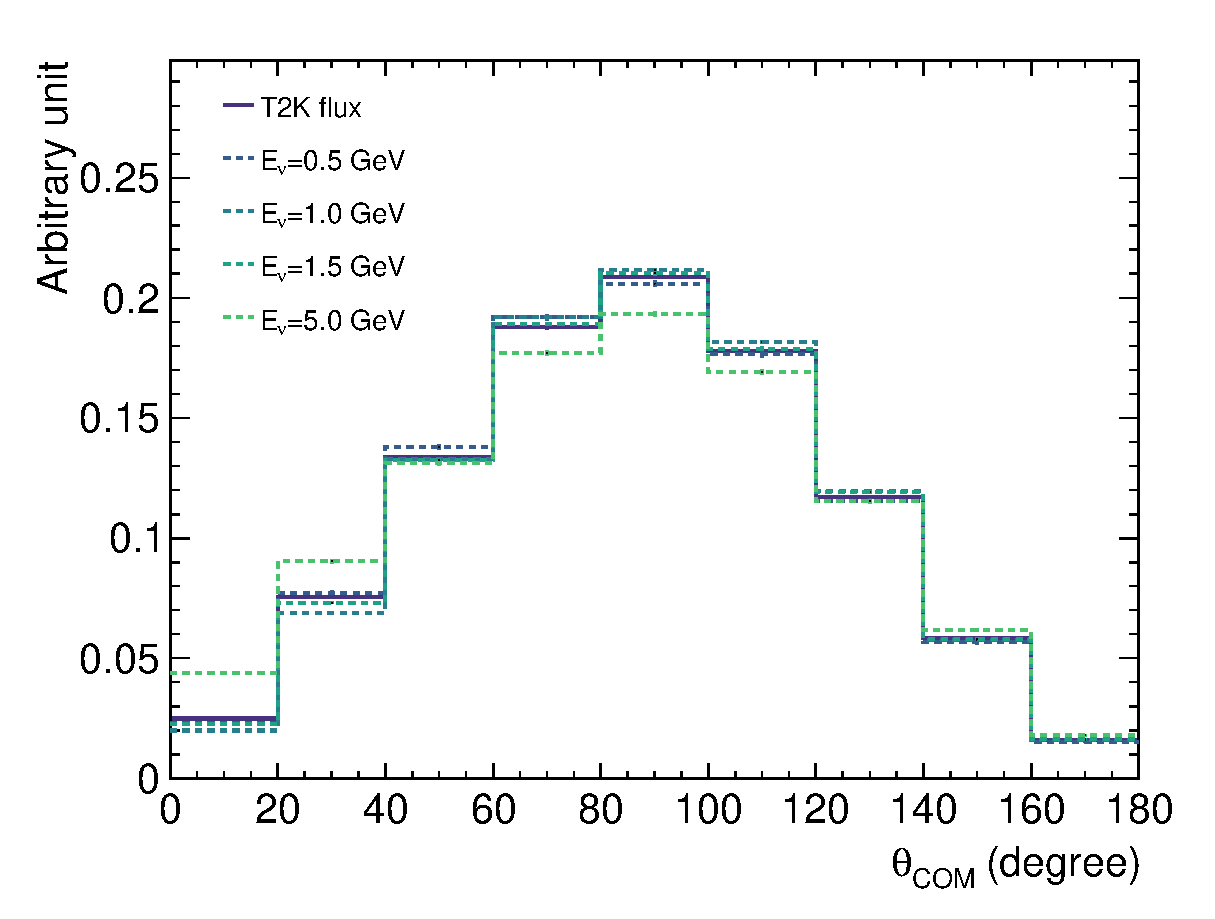
\includegraphics[width=\textwidth]{anorm-monoEnu-less-flux_da_tan.eps}
        \caption{$\numuccopiop$}
        \label{subfig:enu-comp-cc1pi1p}
    \end{subfigure}
        
    \begin{subfigure}[ht!]{\scfigwid\textwidth}
        \centering
        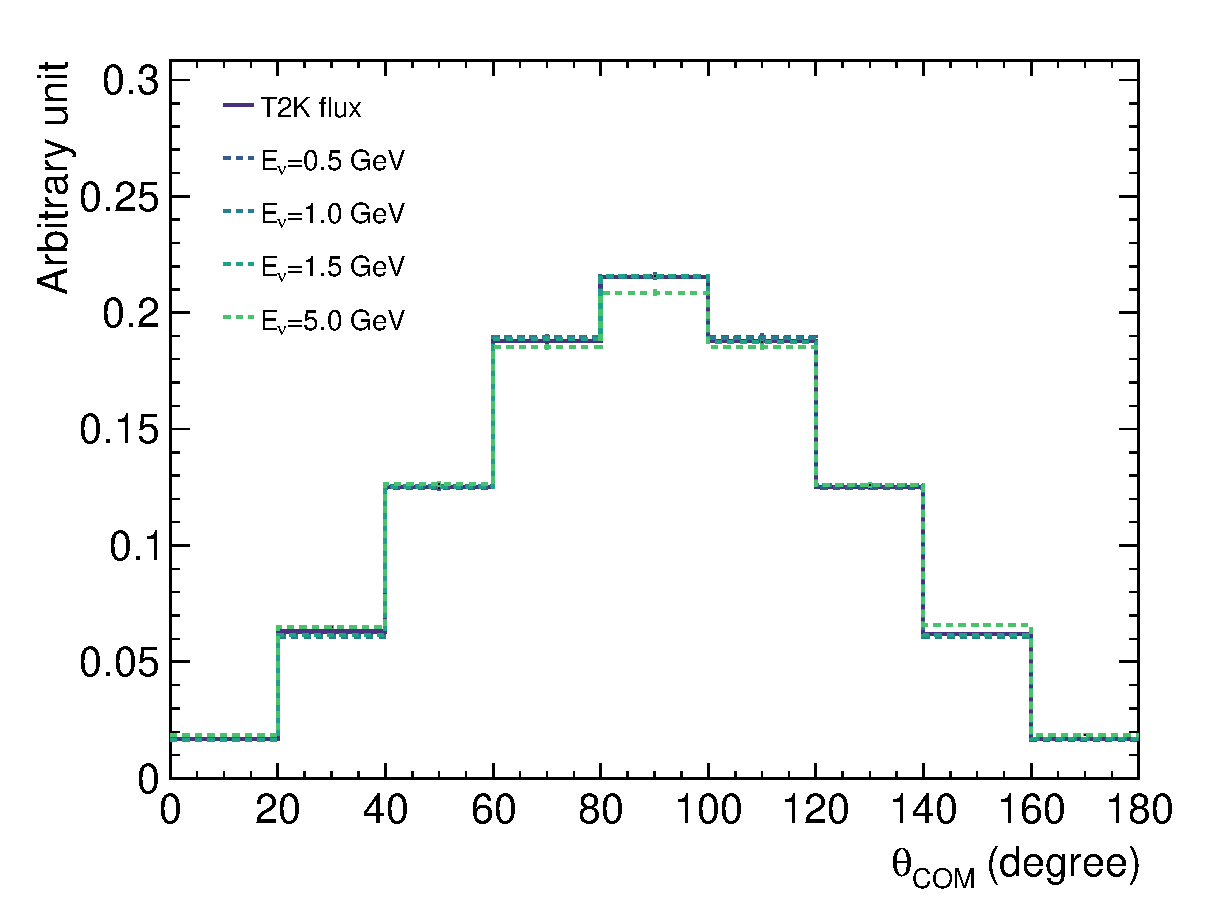
\includegraphics[width=\textwidth]{anorm-monoEnu-less-flux-mode11-_da_tan.eps}
        \caption{$\deltapp$ decay}
        \label{subfig:enu-comp-dpp}
    \end{subfigure}
    \caption{Area normalized comparisons for different $\enu$ fluxes for $\thetacom$.}
    \label{fig:enu-comp}
\end{figure}

Besides $\enu$, another important component in the production of resonances is the part of the $\nu$-N interaction modeling that describes the resonance interaction. 
While $\thetacom$ for a single resonance is largely independent of how the resonance is produced unless there is a strong correlation bewtween the production and decay of the resonance, $\thetacom$ will be affected by the composition of different resonances in the production process. 
As different resonances can have different decay angular distributions and $\thetacom$ does not distinguish between resonances that have the same decay channel, different combinations of resonances in production modelling will change the $\thetacom$ distribution. 
As a proxy to investigate the impact of a change in the resonance production model, the axial mass parameter, $\MA$, was varied to an exaggerated and most likely unphysical extent and the effect is shown in Fig.~\ref{fig:ma-comp}. 
As anticipated, Fig.~\ref{subfig:ma-comp-xsec} demonstrates that varying $\MA$ alters the cross-section.
However, it is reassuring to observe that the shape of $\thetacom$ remains almost identical, as shown in Fig.~\ref{subfig:ma-comp-area}. 

\begin{figure}
    \centering
    \begin{subfigure}[b]{\scfigwid\textwidth}
        \centering
        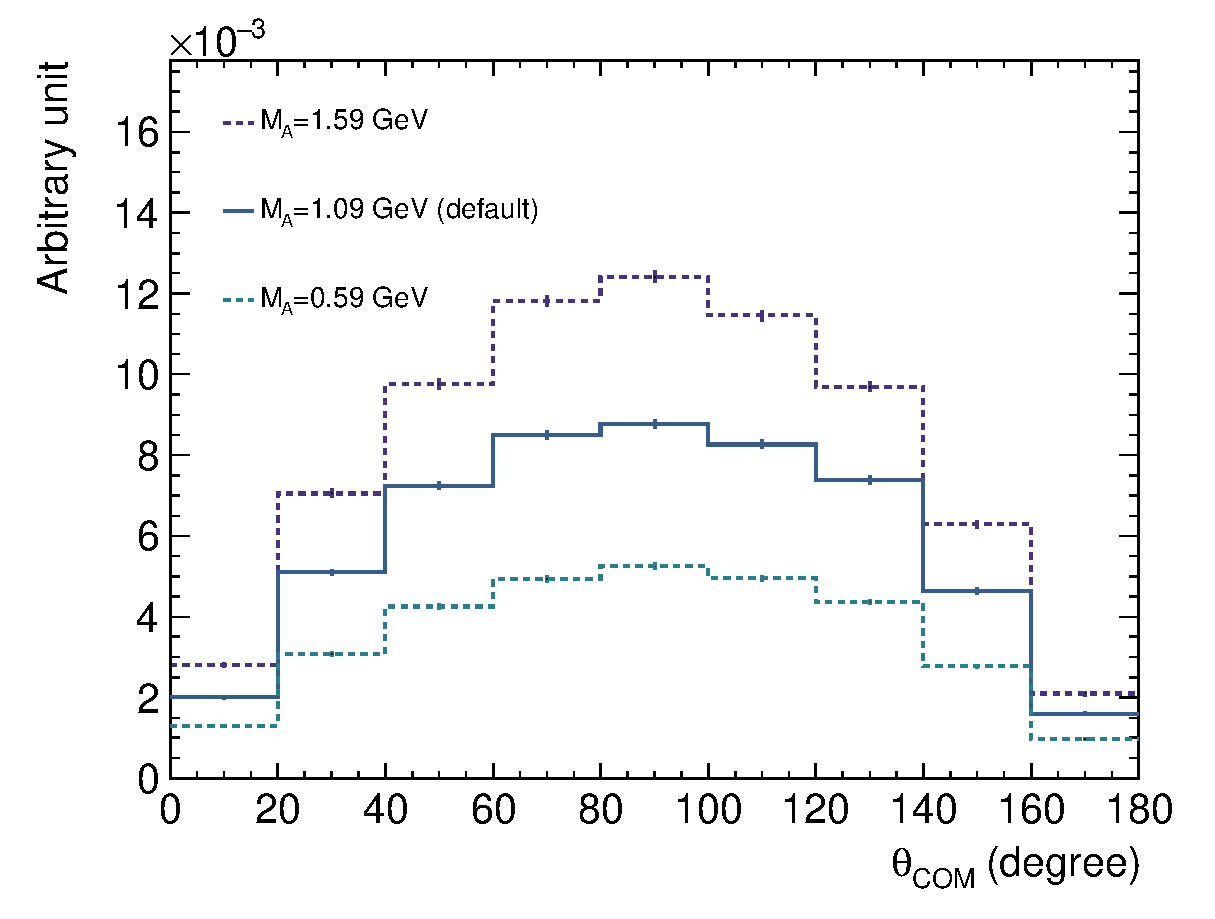
\includegraphics[width=\textwidth]{xnorm-ma_da_tan.eps}
        \caption{cross section normalized}
        \label{subfig:ma-comp-xsec}
    \end{subfigure}
    \begin{subfigure}[b]{\scfigwid\textwidth}
        \centering
        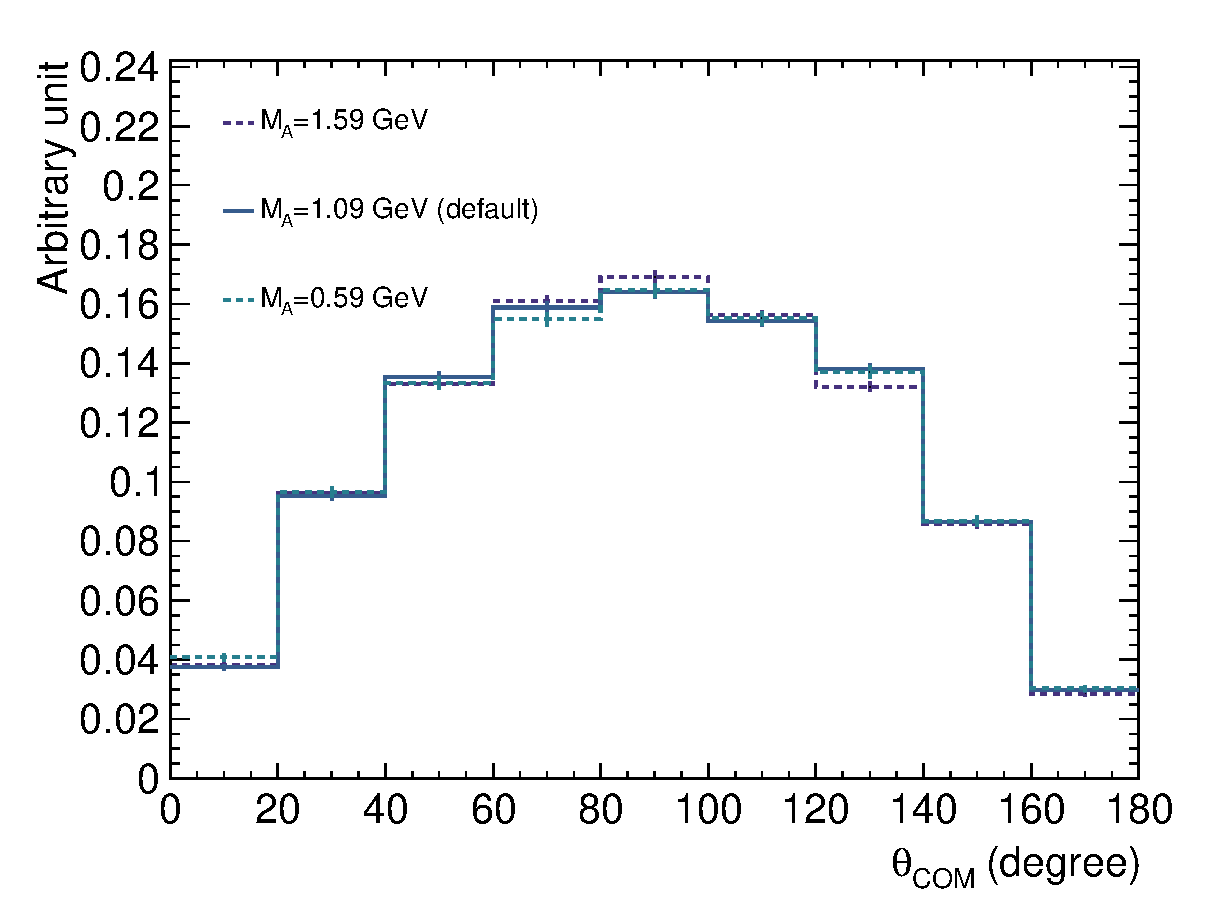
\includegraphics[width=\textwidth]{anorm-ma_da_tan.eps}
        \caption{area normalized}
        \label{subfig:ma-comp-area}
    \end{subfigure}
    \caption{Comparisons for different $\MA$ values with T2K flux. }
    \label{fig:ma-comp}
\end{figure}


\section{Discussion}
\label{sec:dis}
The above simulation studies demonstrate that the COM angle is a novel variable with several advantages, and its measurement will be valuable for studying FSI independently of IS.

Although the analysis focus of $\thetacom$ is on nuclear effects, it is inherently affected by the resonance interaction modelling. 
Fortunately, the $\nu$-N interaction is relatively well-understood, particularly through direct studies of $\nu$-H interactions. 
As a result, future RES modeling is not expected to deviate drastically from current predictions, which are constrained by bubble chamber data.
Even if the RES model were to change significantly, as explored in Fig.~\ref{fig:ma-comp}, the impact on the shape of $\thetacom$ remains minimal, particularly for the T2K flux.
This suggests that FSI models tuned using $\thetacom$, e.g. following the methodology in Ref.~\cite{GENIE:2021zuu}, will continue to be applicable even if the RES model undergoes future updates, thereby enhancing the robustness of such FSI model tuning.

\blue{As noted in Sec.~\ref{sec:com}, the $\thetacom$ distribution is influenced by the production of higher resonances that decay through the same channels as $\deltapp$.
The impact is two-fold.
Firstly, due to general difference of $\thetaR$ from $\thetapidel$, $\thetacom$ would start to deviate from $\thetapidel$ (smeared by FSI), as shown in Fig.~\ref{subfig:enu-comp-cc1pi1p}. 
Although $\thetacom$ is inspired by $\thetapidel$, it is not restricted to the reconstruction or estimation of $\thetapidel$. 
Rather, $\thetacom$ by definition is the superposition of all energetically accessible $\thetaR$, with $\thetapidel$ being the dominant component at low energy.
If all $\thetaR$'s are relatively well understood, a simple theoretically motivated expectation of $\thetacom$ can be obtained by adding the contributions from all possible R according to the relative production ratios.
This simple approach is complicated by the second point - even with a complete understanding of the FSI model, the predicted $\thetacom$ distribution would deviate from measurements due to correlations among different resonance production modes, i.e. the overall $\thetacom$ is not simply a linear combination of the individual $\thetaR$ contributions.
Nevertheless, the influence of higher resonances is minor for low-energy neutrino beams and can be further reduced by applying an upper cut on the COM total energy, ensuring that the selected events predominantly arise from $\deltapp$ decay.
As FSI modeling improves and single-resonance models are refined through constraints from other experiments, the COM total energy cut could be lifted. 
This would enable the full $\thetacom$ distribution to be used for studying correlations and advancing RES modeling.}

The sensitivity of the COM frame to FSI can be leveraged not only to study FSI but also to select events without FSI. 
These events are primarily composed of $\nu$-H interactions, which provide a unique opportunity for precise measurements of the axial current—a feature specific to neutrinos. 
Additionally, a $\nu$-H sample allows for the improvement of $\nu$-H modeling without the complications of IS and FSI, facilitating accurate neutrino energy reconstruction. 
These advantages have driven significant efforts to develop techniques for selecting a high-purity $\nu$-H sample, as seen in Ref.~\cite{Lu:2015hea,MINERvA:2023avz,Baudis:2023tma}.
While Ref.~\cite{Baudis:2023tma} and Ref.~\cite{MINERvA:2023avz} focuses on neutrino and antineutrino pion-less events respectively, Ref.~\cite{Lu:2015hea} applies to the same event topology as the COM total energy. 
Preliminary studies have shown that applying a cut on COM energy can remove events with minimal transverse momentum imbalance, which could be combined with cuts on $\dptt$ and $\dpt$ to create a high-purity $\nu$-H sample. 
This approach will be explored further in future studies.

Although the COM angle shares a similar reconstruction target with the Adler angle, there are key differences, as discussed in Sec.~\ref{sec:ana}. 
While these differences may appear minor, the conceptual distinction makes tuning the FSI model using the COM angle more adaptable to future developments. 
Furthermore, the analyses presented here are based on true information without any realistic fluctuations, meaning that challenges related to reconstruction—particularly those involving neutrino energy for the Adler angle—are not considered. 
Therefore, the full potential of the COM angle will be better realized in a cross-section measurement that accounts for these complexities.

\section{conclusion}
This study introduces a novel set of variables—the COM angle and total energy.
These variables offer several advantageous properties, motivating their use in future cross-section measurements.
These measurements have the potential to significantly improve our understanding and modeling of FSI processes in neutrino-nucleus interactions, thereby contributing to more accurate neutrino cross-section predictions.

\section{Introduction}
There have been tremendous efforts to measure Charge-Parity (CP) violation in the neutrino sector by long-baseline experiments. 
Massive detectors, like Hyper-Kamiokande (Hyper-K) or the far detector of the Deep Underground Neutrino Experiment (DUNE), are proposed or being built. 
The measurement of $\dcp$, the CP violating phase, will have such large statistics that the uncertainties will be systematics dominant. 
It is pivotal to build more advanced models or to constrain existing models to provide more accurate predictions to maximize the physics potential of the coming experiments.
To gain a better understanding of the complicated neutrino-nucleus interactions, experiments with new and sophisticated detectors have started running, for example, the Tokai-to-Kamioka (T2K) experiment has upgraded the near detector and has started data collection in June 2024. 
Meanwhile, the Short-baseline Neutrino Detector (SBND) has also started running with a new ??? detector. 
These new detectors are much more capable than their predecessors. 
For example, the Super Fine-Grain Detector (SFGD) has a much-improved proton detection in terms of lower threshold, better resolution and higher efficiency. 
This advancement opens up possibilities for measurements of new useful variables. 
As the DUNE beamline ha a broad spectrum, it has a large contribution from resonance production, comparable to the quasi-elastic interaction.
Hence, it will be timely to explore new ideas with pions in the final states expecting the large influx of data. 

One effective method to improve our models is to constrain the parameters using existing data via tuning. 
There have been successful examples of observing better data-Monte Carlo (MC) agreement (cite cite cite) after tuning existing models using various combinations of measurement across experiments. 
However, as the neutrino-nucleus interaction is a convolution of multiple processes, namely the nucleon Initial State (IS), the neutrino-nucleon interaction and the Final State Interactions (FSI), many of the variables experience the impacts of all processes, thereby making it difficult to study the different models individually. 
Especially the nuclear effects, i.e. IS and FSI, are within the nucleus and cannot not be observed directly by present-day detectors. 
Hence, they contribute as a major source of systematic uncertainties. Cleverly construct variables, like the Transverse Kinematic Imbalance (TKI) (cite) variables or the Generalized Kinematic Imbalance (GKI), are sensitive to the nuclear effects. Past measurements have yielded fruitful model constraints [cite various TKI tuning paper]. 
While TKI is sensitive to both IS and FSI, new variables, like p_long [cite], are constructed to be particularly sensitive to a certain characteristic of the nuclear effects, in this case, the removal energy. 
Having more specialized measurement, like p_long, will be beneficial as it provides a more dedicated channel to fine tune our models. 

So far, all these variables are subject to both IS and FSI, except $\dat$, which is sensitive only to FSI but is affected by small uncertainties in the neutrino direction. As it is highly beneficial to have variables sensitive to a particular feature of the nuclear effects independently from others and in view of the enhanced detection capabilities and future measurements with pion in the final states. In this work, the author proposes a new set of variables, namely the centre-of-momentum (COM) variables in Charge Current Single Pion ($\ccopi$) events. The COM variables are capable of differentiating different FSI models regardless of IS models, thereby making dedicated studies on FSI possible. This work will elaborate on the concept of COM, followed by analysis results demonstrating the FSI differentiation power and the independence from IS. 

\section{COM}
When the neutrino possesses enough energy, it can excite the nucleon into a resonance, most commonly the $\deltapp$. This is the so-called resonance (RES) interaction. The resonance has a finite momentum from the RES interaction. However, it is extremely short-lived and decays quickly before exiting the nucleus, via 
\begin{equation}
	\deltapp \rightarrow \pip + \pr,
\end{equation}
as shown on the left in Fig.~\ref{COM-diagram}. The $\deltapp$ direction in the lab frame is chosen to be the x-axis, which coincides with the x’-axis of the $\deltapp$ rest frame. The angle, $\theta$, is defined with respect to the x-axis. As this is a two-body decay, the $\pdd$ can be obtained by summing $\ppi$ and $\ppr$, which can then be used to boost the system back to its rest frame. In this frame, the kinematics are exactly, given the rest mass of the resonance, except $\theta$ is chosen according to an underlying distribution, which are given by many models [cite MK etc]. 


So far the discussion on the resonance decay is completely general and hence it is applicable to and can be crosschecked by many other experiments, [hadron-nucleon collision?] There are properties specific to neutrino experiments. Firstly, the resonance is produced by neutrino interacting with a nucleon, so both vector and axial currents are present. Secondly, the interaction takes place inside the nucleus. This work explores the latter in greater depth, while the application of COM to the former will be pursued in future works. 


As the pion and the proton propagate out of the nucleus, they experience FSI, leading to modified kinematics, $\ppipp$ and $\pprp$, measured in the lab frame. Thus, the sum of measured momenta, $\psum = \ppipp + \pprp$, is in general not equal to $\pdpp$ anymore. Regardless, it is possible to boost the system to the centre-of-momentum (COM) frame using $\psum$, as shown on the right in Fig.~\ref{COM-diagram}. Similarly, $\thetap$ is in general different from $\theta$. In the absence of FSI, the COM frame coincides with the $\deltapp$ rest frame. Hence, the strength of FSI controls the extent to which $\ftp$ deviates from $\ft$. In practice, the measured $\ftp$ can be used as a probe to study FSI. Since the $\ft$ is a property of $\deltapp$ in its rest frame, it is independent of the $\deltapp$ momentum, and thus of the neutrino energy and of IS. Critically, $\ftp$ differs from $\ft$ only by FSI, which by definition is also independent of neutrino energy and of IS. As a result, $\ftp$ inherits these desired independences. 

FIG-COM-diagram

Conceptually, the COM angle might seem similar to Adler’s angle. However, there are key differences. Most importantly, the COM frame is reconstructed entirely based on hadron kinematics, while the Adler frame is built based on leptonic kinematics assuming stationary nucleons. Hence, the reconstruction of the Adler frame is affected implicitly by IS, while the hadronic variables are affected by FSI. Hence, Adler’s angle, a hadronic variable in the Adler frame, will be affected by both IS and FSI. Moreover, the need to reconstruct the neutrino energy makes variables in the Adler frame susceptible to the neutrino flux uncertainties, one of the largest systematics in neutrino experiments. [cite t2k result to prove]

To have a concise discussion on the main concept, this work focuses on $\deltapp$, as it is the dominant type from the T2K beam and it is also one of the most common types in DUNE [need to cite to prove both], but the idea is equally applicable to other resonances and implementations can be easily generalized. 

\section{Analysis result}
As there are no measurements of the COM angle yet, Monte Carlo studies have been performed to investigate its proclaimed advantages. Monte Carlo samples using \genie are produced using both the T2K and MINERvA beams and targets. Multiple \genie tunes are used in comparison. The model details for the different tunes are summarised in Table~\ref{tab:GENIE-TUNES}. Charge Current (CC) events with one pion and proton in the final states are selected to produce the plots.

TABLE:GENIE-TUNES



As shown in Fig.~\ref{fig:fsi-comp} (a), switching FSI on and off has a large impact on the $\tp$ cross-section measurement as expected. More importantly, Fig.~\ref{fig:fsi-comp} (b) demonstrates that a change of the underlying FSI model from hA (10a) to hN (10b) leads to a distinguishable shape change in the $\tb$ cross-section, thereby showcasing the FSI model discrimination power of $\tp$.

\begin{figure}
    \centering
    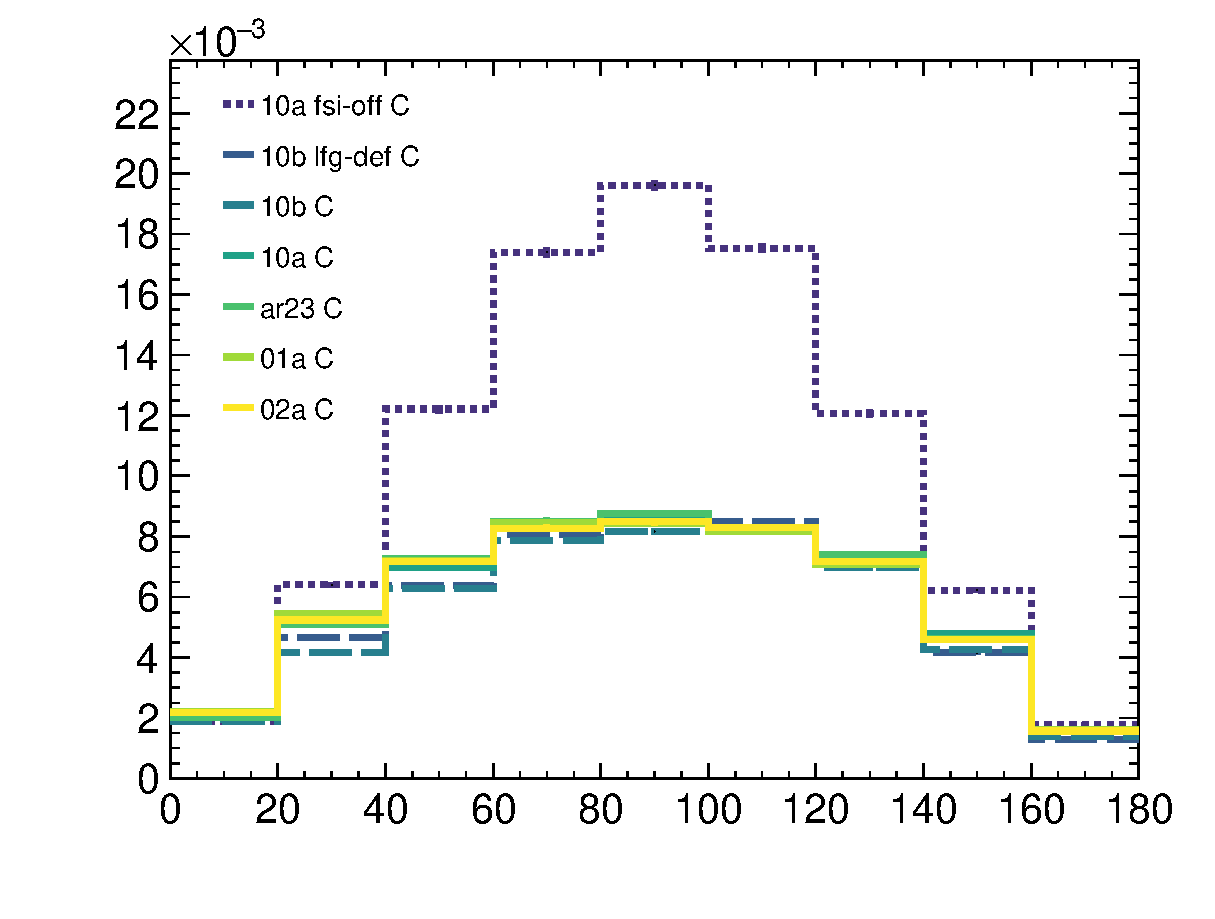
\includegraphics[width=\linewidth]{xnorm-mod-wfsioff-da.eps} \\
    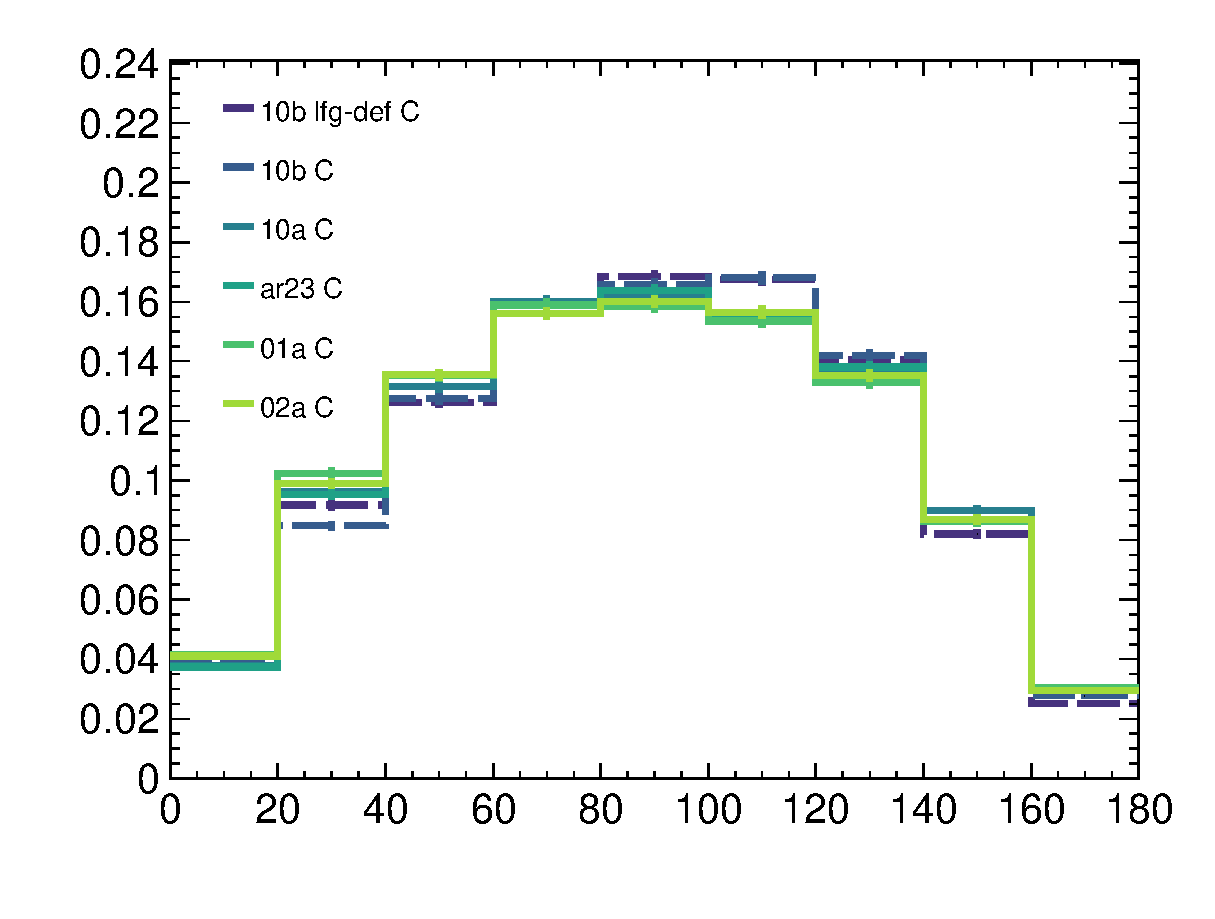
\includegraphics[width=\linewidth]{anorm-mod-nofsioff-da.eps}
    \caption{(a) Comparing FSI on/off xsec norm for 10a, (b) Comparing 10a and 10b (area normed)}
    \label{fig:fsi-comp}
\end{figure}

Another advantage of $\tb$ lies in its independence of IS. One ultimate test for this is to compare the cross-section shape of $\nu-C$ with FSI on and off with that of $\nu-H$. The $\nu-H$ interaction has no nuclear effect at all. The $\nu-C$ with FSI off shows the impact of IS, including removal energy for carbon and Fermi motion. The $\nu-C$ with FSI on has the full nuclear effects, both IS and FSI. As shown in Fig.~\ref{fig:ch-comp} (a), FSI has the strong impact on the cross-section shape as expected. The almost coincidence of the $\nu-H$ curve and the $\nu-C(fsi-off)$ curve is strong evidence supporting the claimed independence from IS of $\tp$.

\begin{figure}
    \centering
    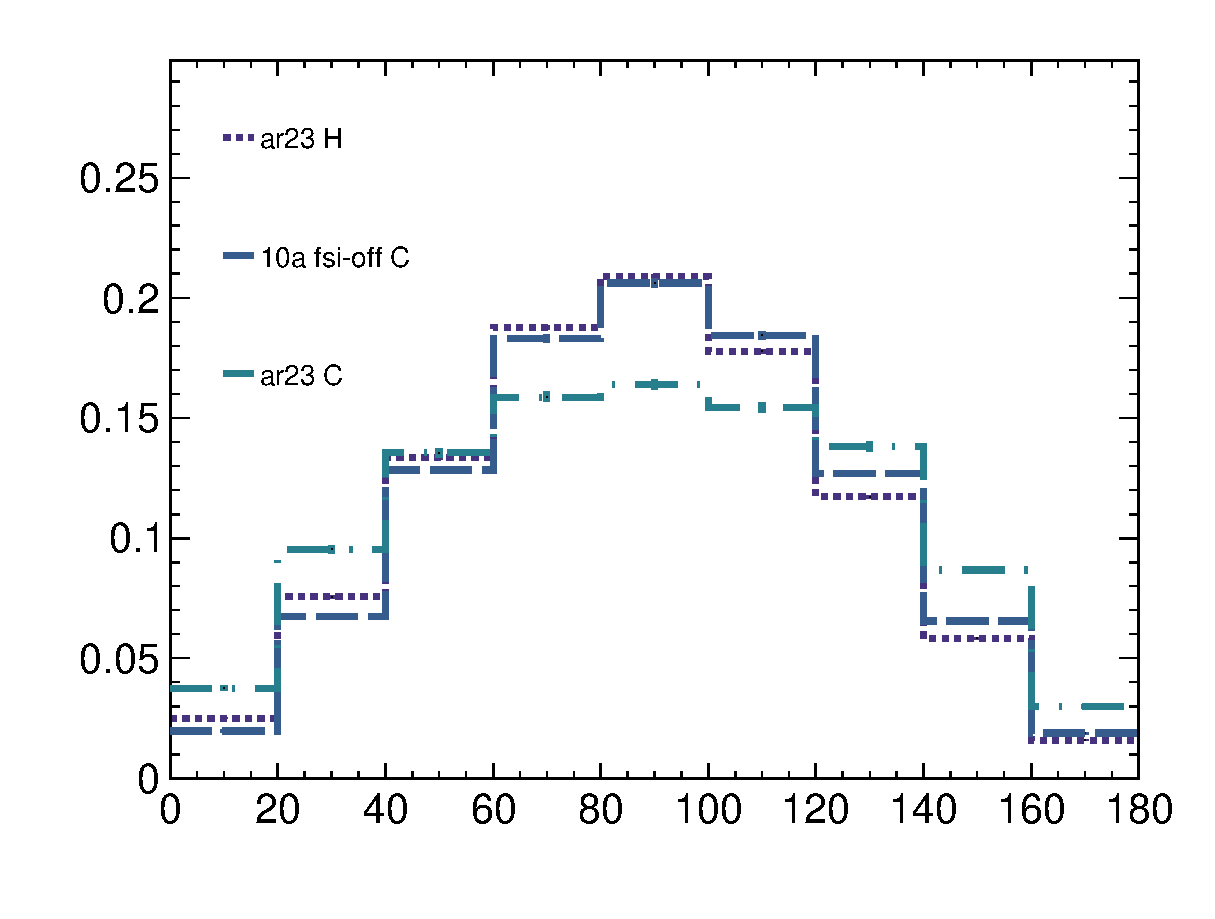
\includegraphics[width=\linewidth]{anorm-ch-da.eps}     \\
    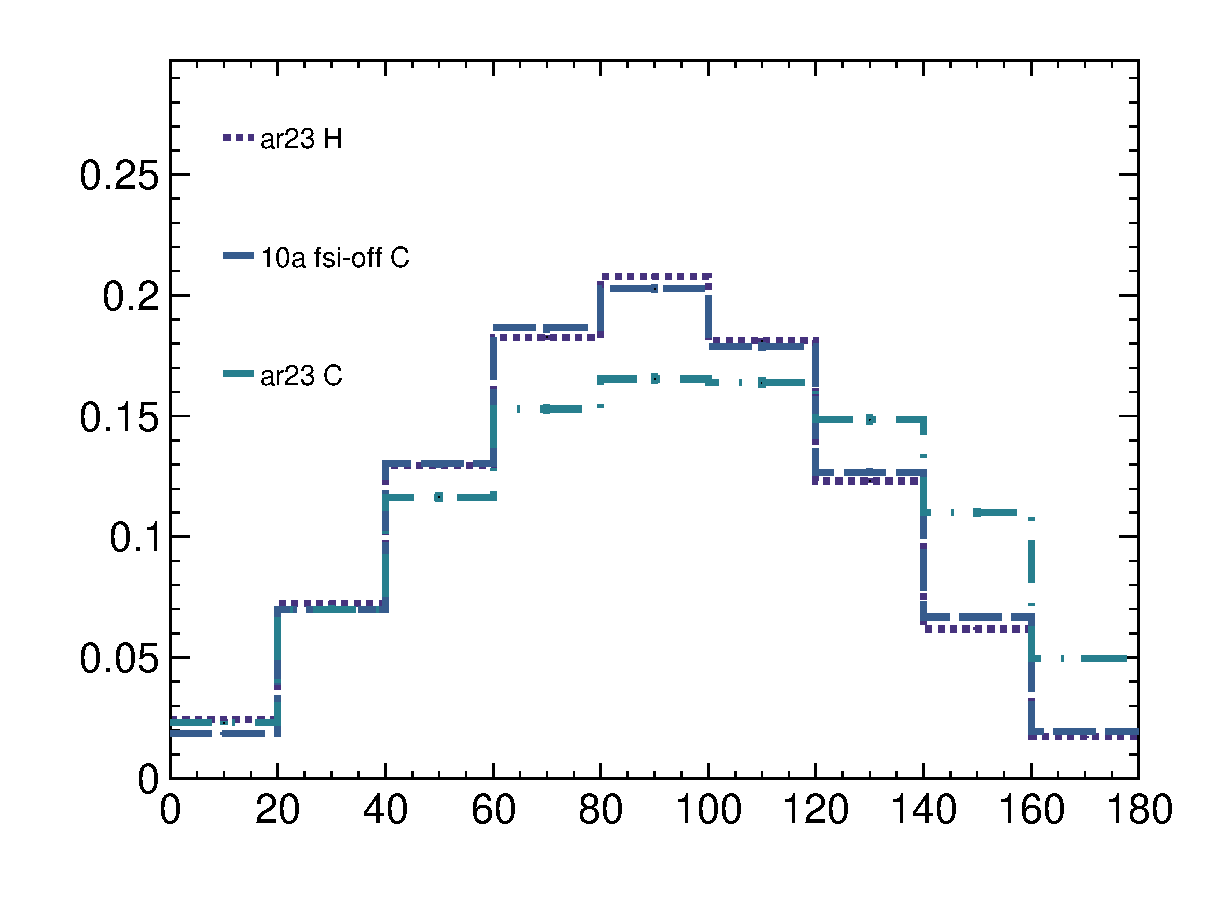
\includegraphics[width=\linewidth]{anorm-ch-adt.eps} 
    \caption{Anorm – nuH nuC(fsi-off) nuC(fsi-on) comparison. (a) $\tp$ (b) $\adt$.}
    \label{fig:ch-comp}
\end{figure}


Since $\tp$ is conceptually close to the Adler’s angle except that Adler’s angle has the additional influence from IS. In Fig.~\ref{fig:ch-comp} (b), the $\nu-H$ curve and the $\nu-C(fsi-off)$ curve are just as close to each other as in Fig.~\ref{fig:ch-comp} (a), suggesting that despite the dependence on IS, IS effectively does not distort the $\adt$ shape appreciably. This could put the claimed IS independence of $\tp$ in question, as it could be due to relatively small impact from IS. To verify this claim, a further stress test is performed. The removal energy of carbon is varied significantly, even to unphysical extents, to just observe its impact on the shape of $\tp$ and $\adt$. The result is shown in Fig.~\ref{fig:ermc-comp}.

\begin{figure}
    \centering
    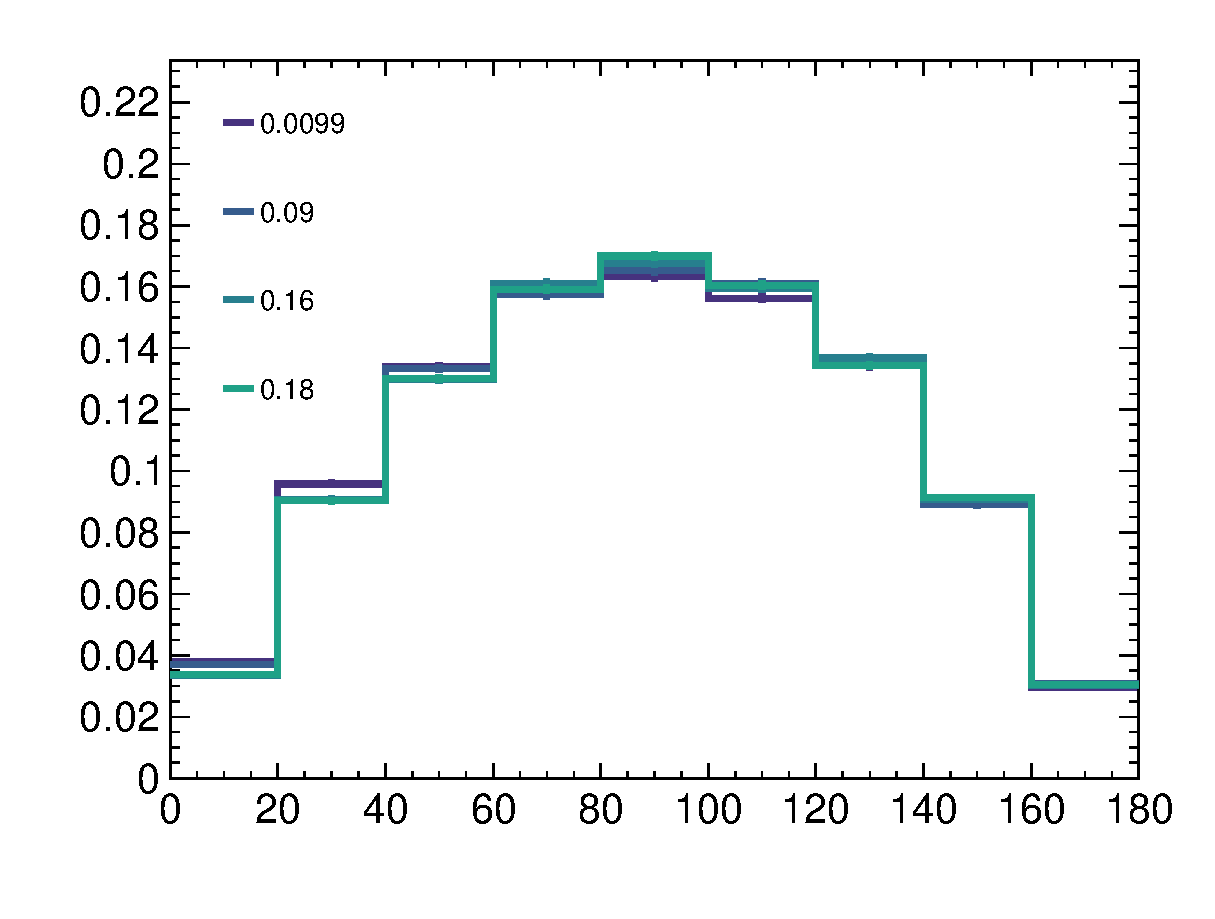
\includegraphics[width=\linewidth]{anorm-nuc-da.eps}\\
    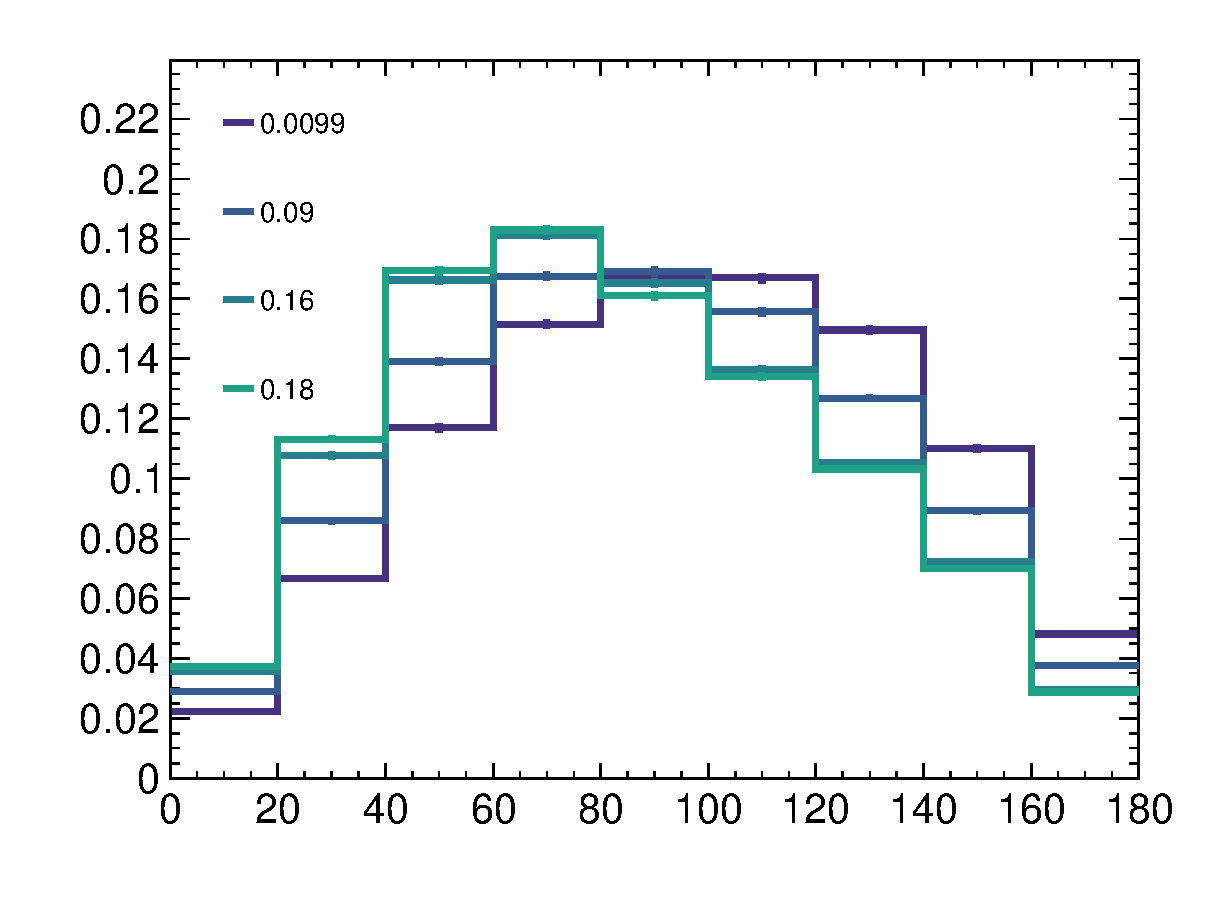
\includegraphics[width=\linewidth]{anorm-nuc-adt.eps}
    \caption{Anorm – Ermc comp (a) $\tp$ (b) $\adt$}
    \label{fig:ermc-comp}
\end{figure}


It is apparent in Fig.~\ref{fig:ermc-comp} that regardless of any changes in Ermc, $\tp$ is not affected at all. Meanwhile, there is a clear shift in the $\adt$ peak and a gradual change in its shape as well. This affirms the robust IS-independence of $\tp$ and the IS-dependence of $\adt$ as conjectured.
An additional desired property of $\ftp$ is its independence on the neutrino energy. As shown in Fig.~\ref{fig:enu-comp}. On the whole, the shapes of $\ftp$ for $\enu$ between $0.5\gev$ and $2.0\gev$ are largely similar over a large portion of the range. However, the deviation becomes larger at small angles. When $\enu$ increases to $5\gev$, the increase in the small angle region is apparent. It is likely due to the onset of the next doubly positive resonance. (which one?) If the selection is restricted to $\deltapp$, it is reassuring to see that the different curves collapse to one, demonstrating the independence from $\enu$. 

\begin{figure}
    \centering
    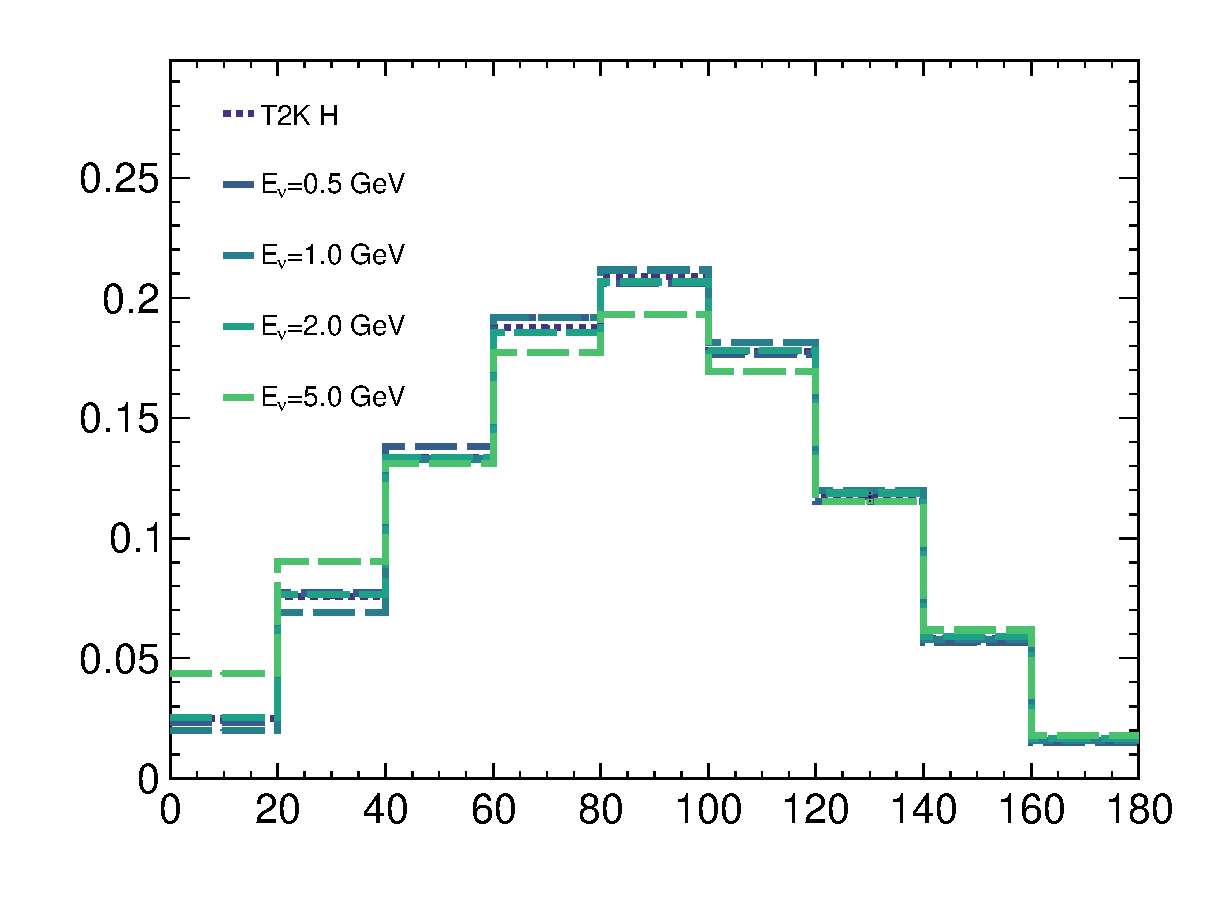
\includegraphics[width=\linewidth]{anorm-monoEnu-less-flux-da.eps}
    \caption{Anorm different enu fluxes ---- SHOULD PLOT ONE WITH MODE==11 ON FOR THE DIFFERENT ENU TO REMOVE HIGHER RESONANCE.}
    \label{fig:enter-label}
\end{figure}

\section{Discussion}
Through the multiple simulation studies, it has been demonstrated that the COM angle is a new variable with several strengths and its measurement will be valuable in studying FSI independently from IS. This discussion so far has focused on IS and FSI, but as $\deltapp$ is produced in RES, it is naturally affected by the modelling of $\nu$-N interaction. Fortunately, the $\nu$-N interaction is relatively better understood by directly studying $\nu$-H interactions. Hence, future RES modelling would not have drastically different predictions from the current one constrained by the bubble chamber data. To examine the impact of a change in the RES modelling on $\ftp$, the axial mass parameter is changed in steps. While it is expected that changing $MA$ will change the cross section, it is encouraging that the shape of $\ftp$ remains unchanged, as shown in Fig.~\ref{fig:ma-comp}. Hence, FSI models tuned using $\ftp$ will remain applicable even if the RES model is updated in the future, thereby enhancing the usefulness of an FSI model tuning. 

\begin{figure}
    \centering
    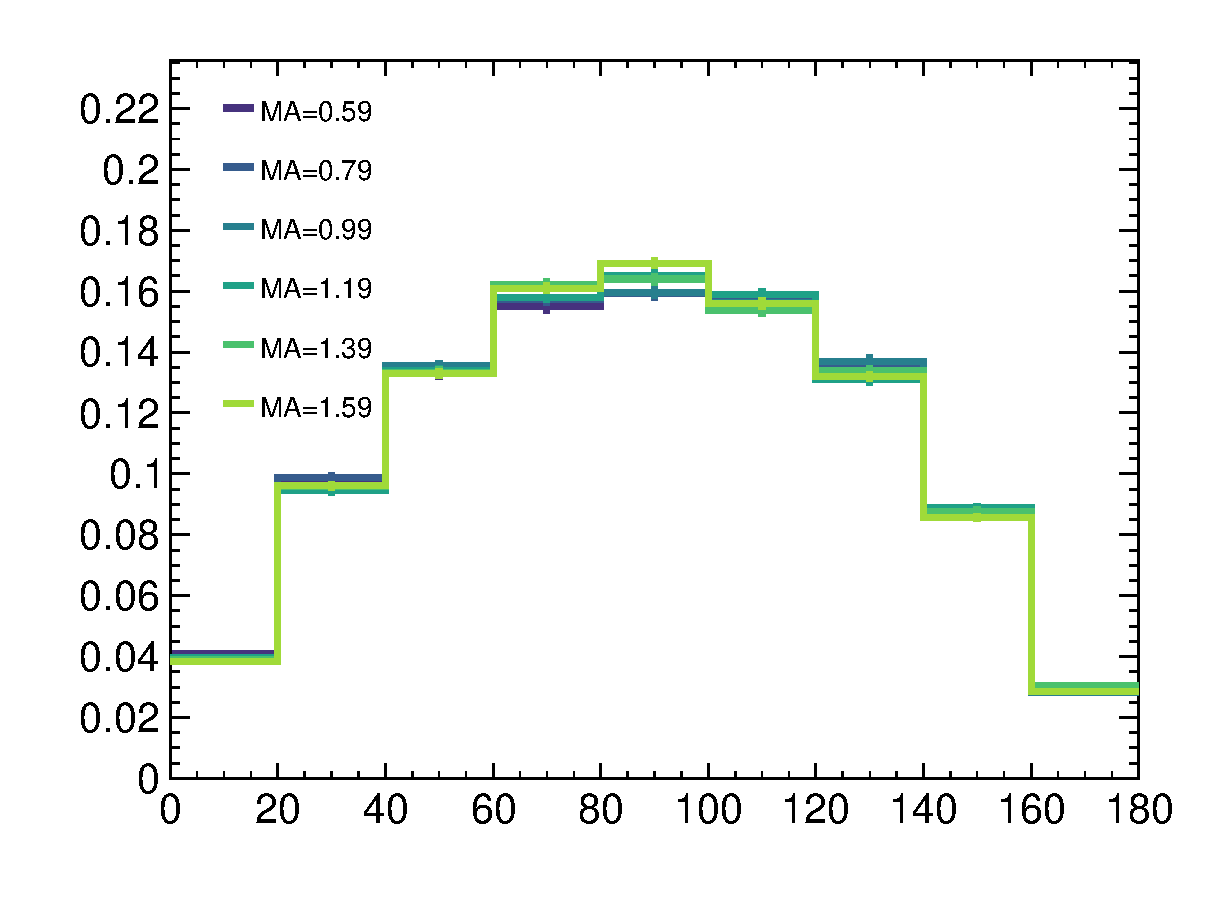
\includegraphics[width=\linewidth]{anorm-ma-da.eps}
    \caption{MA COMP xsec norm and anorm. }
    \label{fig:ma-comp}
\end{figure}

While $\ftp$ is relatively immune to change in $MA$, it might be affected considerably by added correlation between different resonances as hinted in the previous section in Fig.~\ref{fig:enu-comp}, where it is apparent that the next resonance has raised the low angle region of $\ftp$. As \genie does not handle resonance correlations, it will be interesting to study its impact in other generators in future works.
The sensitivity of the COM frame to FSI can not only be used to study FSI, but also to select events without FSI. These events are composed mainly of $\nu$-H interactions, which is the only venue to have a precise measurement of the axial current, unique to neutrinos. Moreover, a $\nu$-H sample offers the opportunity to further improve $\nu$-H modelling without the complications of IS and FSI, which additionally allows precise reconstruction of the neutrino energy. Its importance has sparked many efforts to invent techniques to select a high purity $\nu$-H sample, cite[dptt, Minerva, plong]. While Ref.~\cite[Min,plong] focuses on pion-less events, Ref.~\cite[dptt] is applicable to the same event topology of the COM total energy. A preliminary study has shown that a cut on COM E can cut away events with little transverse momentum imbalance, so it could be used in conjunction with cuts on $\dptt$ and $\dpt$ to produce a high purity $\nu$-H sample. It shall be studied in greater depth in future works.
While the COM angle has a similar reconstruction target as the Adler angle, they have important differences as shown in Sec.~\ref{sec:ana}. Although the difference might seem relatively small, the conceptual difference makes tuning FSI model using the COM angle more future-proof. Besides, the analyses presented are based on true information without smoothing, where difficulties and implications of reconstruction are absent, which can be significant for the neutrino energy required for the calculation of Adler angle. Hence, the full potential of the COM angle will be better demonstrated in a cross-section measurement that takes into consideration all of these complications.
\section{conclusion}
This work has introduced a new set of variables, the COM angle and total energy. They have multiple desired properties, thereby motivating cross section measurements of these variables, which could help to significantly improve our understanding and modelling of FSI in neutrino-nucleus interactions. 



\minitoc